\section{Technical Approach}\label{sec:technical}
\begin{figure*}[htbp]
	\centering
	\begin{subfigure}{0.3\textwidth}
	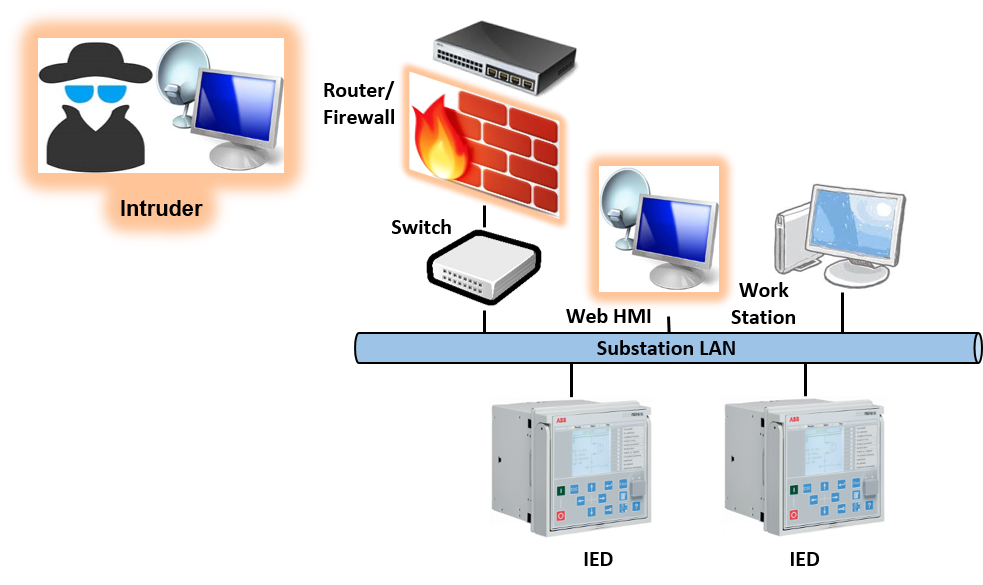
\includegraphics[width=\textwidth]{A-model.png}
	\caption{}\label{sfig:model-A}
	\end{subfigure}
	\begin{subfigure}{0.14\textwidth}
	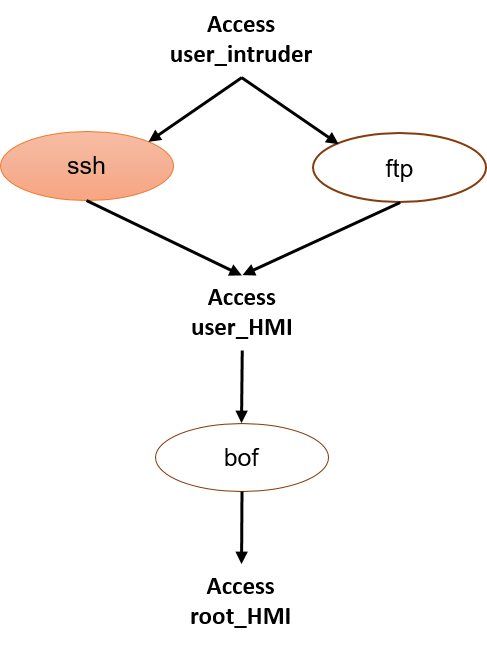
\includegraphics[width=\textwidth]{A-graph.png}
	\caption{}\label{sfig:graph-A}
	\end{subfigure}
	\begin{subfigure}{0.26\textwidth}
	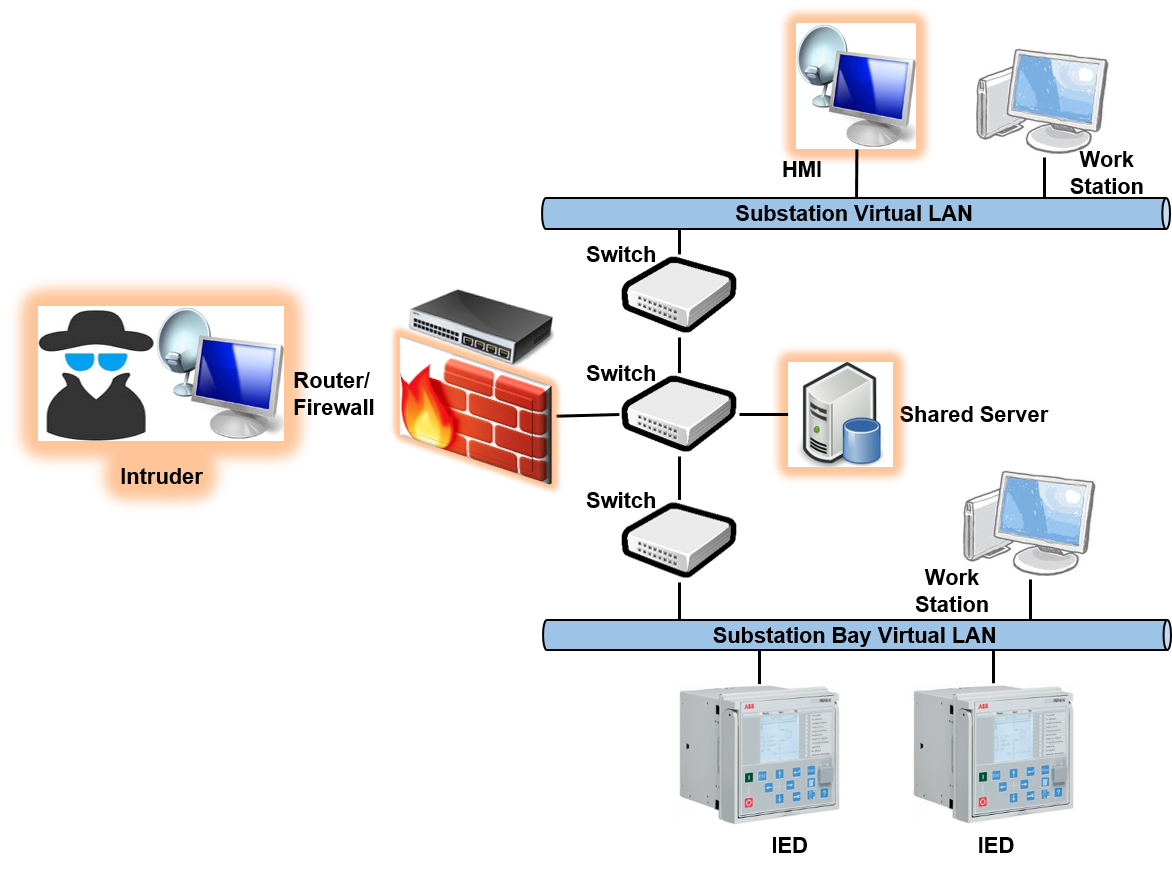
\includegraphics[width=\textwidth]{B-model.png}
	\caption{}\label{sfig:model-B}
	\end{subfigure}
	\begin{subfigure}{0.16\textwidth}
	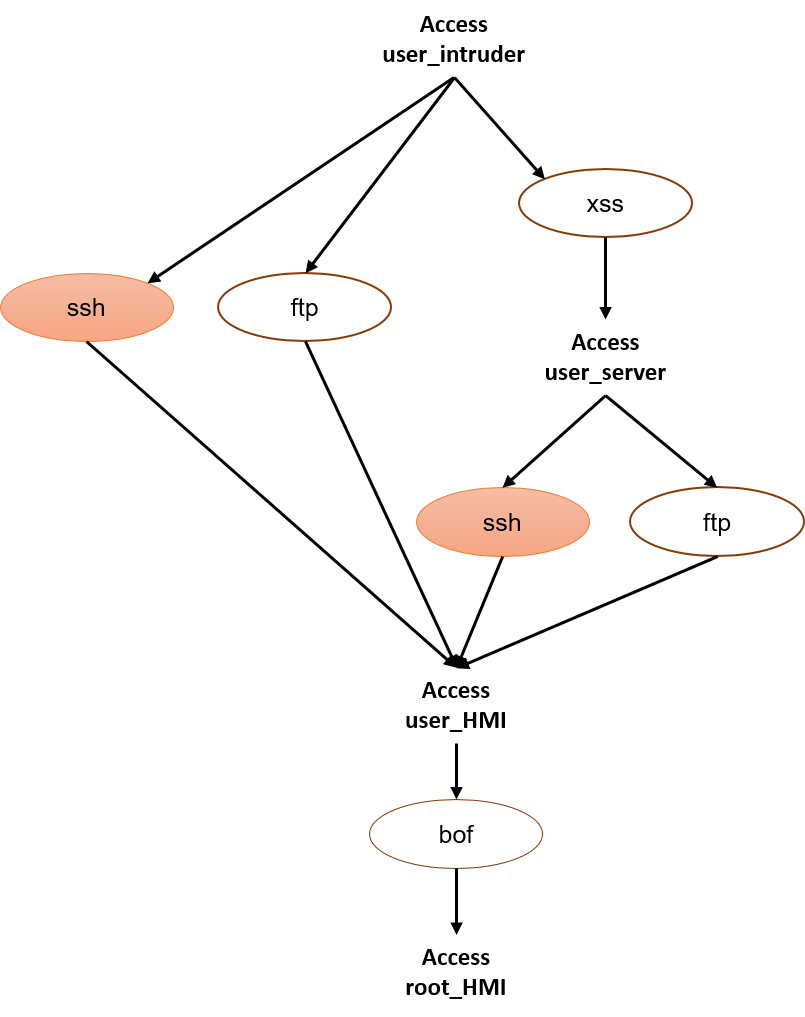
\includegraphics[width=\textwidth]{B-graph.png}
	\caption{}\label{sfig:graph-B}
	\end{subfigure}
	\begin{subfigure}{0.3\textwidth}
	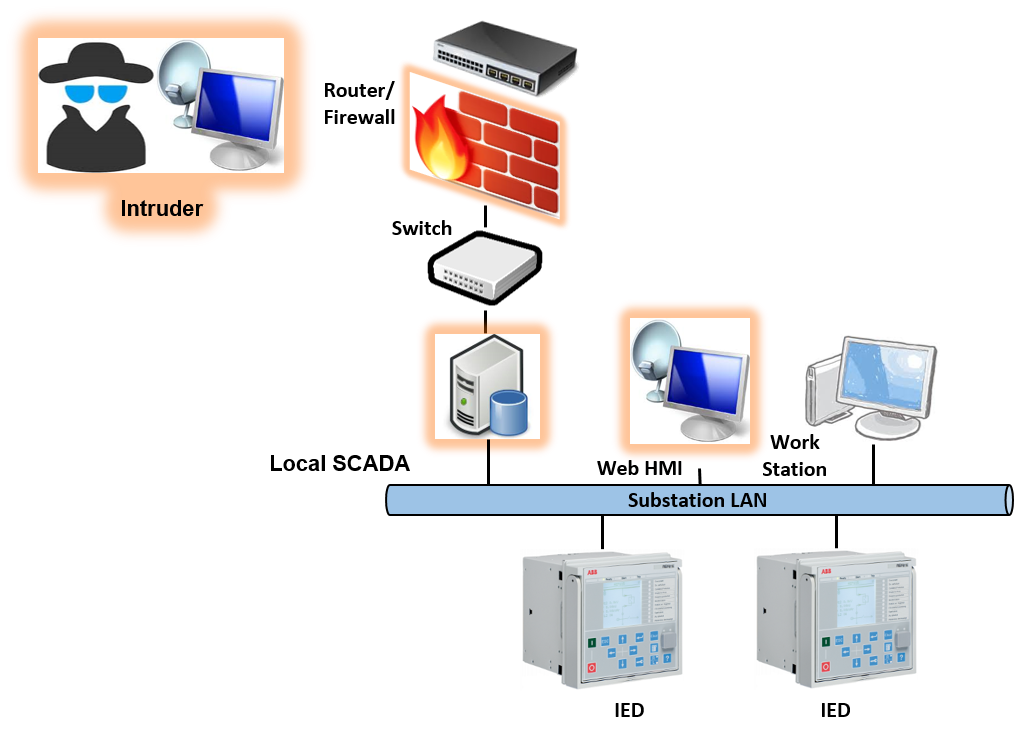
\includegraphics[width=\textwidth]{C-model.png}
	\caption{}\label{sfig:model-C}
	\end{subfigure}
	\begin{subfigure}{0.12\textwidth}
	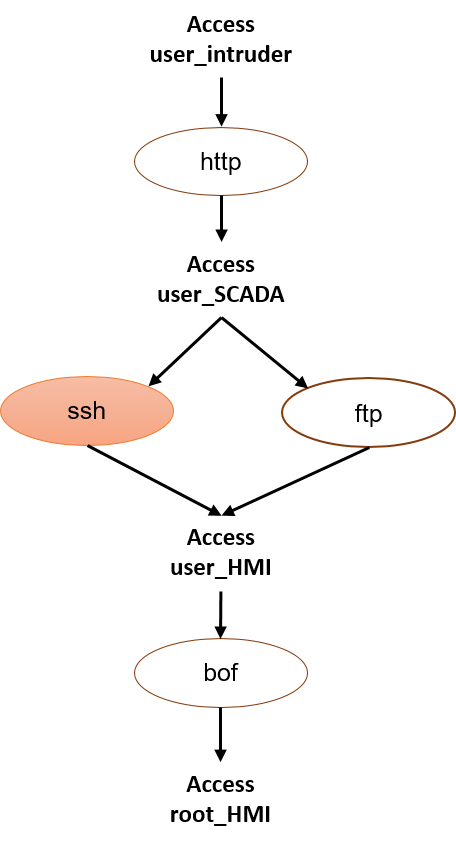
\includegraphics[width=\textwidth]{C-graph.png}
	\caption{}\label{sfig:graph-C}
	\end{subfigure}
	\begin{subfigure}{0.33\textwidth}
	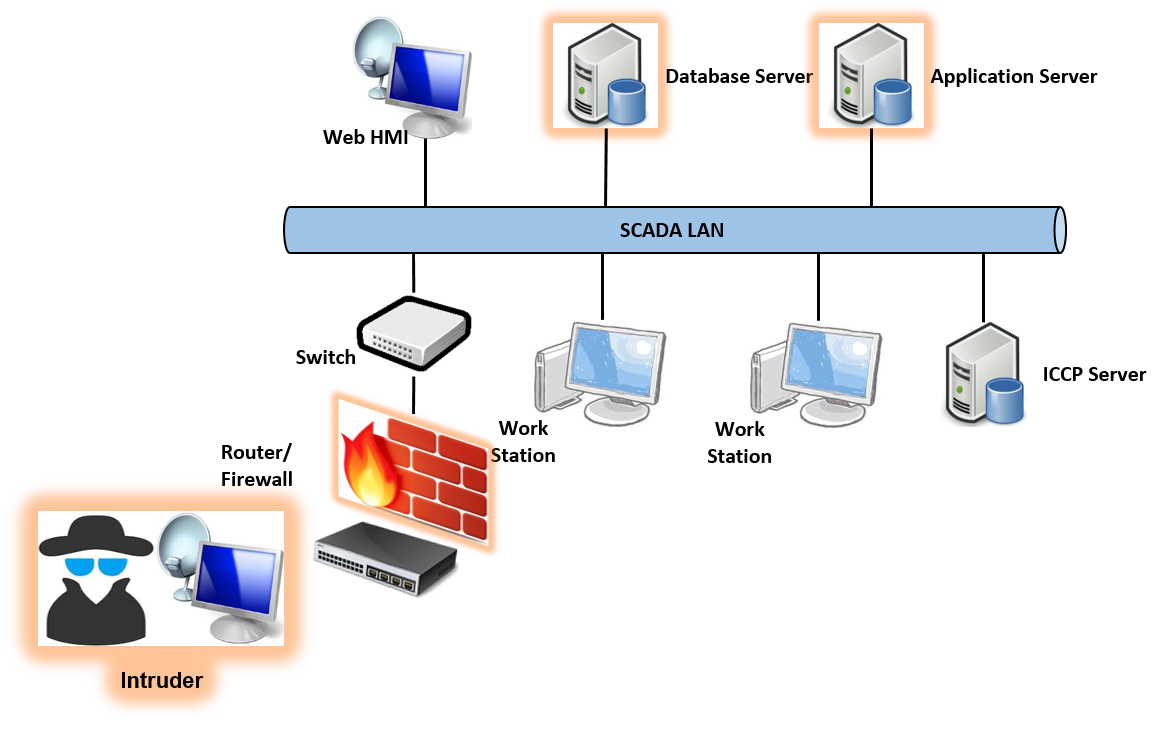
\includegraphics[width=\textwidth]{CC-model.png}
	\caption{}\label{sfig:model-CC}
	\end{subfigure}
	\begin{subfigure}{0.12\textwidth}
	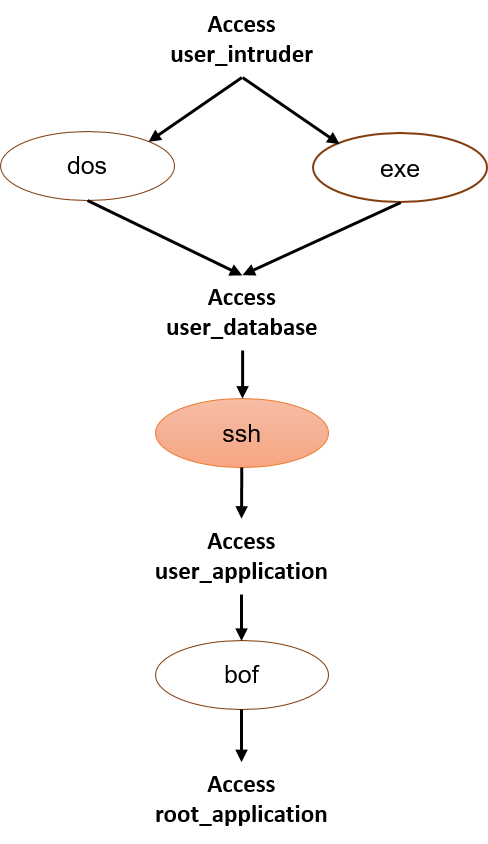
\includegraphics[width=\textwidth]{CC-graph.png}
	\caption{}\label{sfig:graph-CC}
	\end{subfigure}
	\caption{Cyber intrusion scenarios in Substation and Control Center LAN Models and the corresponding attack tree representation.}
\end{figure*}
The proposed security assessment of the power system consists of two parts: (\textit{i})vulnerability assessment of the SCADA system associated with the grid and (\textit{ii}) evaluating vulnerabilities in the physical power system. The net impact of a cyber attack on the SCADA system is therefore evaluated as the combined impact on the cyber system and the physical power system. Each of the system model is discussed in this section.
\subsection{Cyber system model}\label{sec:cyber}
The cyber system model consists of the evaluation of probability of successfully exploiting the vulnerabilities which has been detailed in Section~\ref{sec:prelim} and the calculation of time to compromise a vulnerability. The time to compromise known and zero day vulnerabilities are evaluated in~\cite{mcqueen}. These are denoted by $T(v_k)$ and expressed as an exponential function of $k$ which represents the capability of the intruder in identifying a possible exploit to a vulnerability. In this paper, four possible skill levels are considered for the intruder with $k=10,2,1,0.01$. These intruders are identified as expert, professional, intermediate and amateur level adversaries respectively. The time to compromise decreases exponentially with increase in skill level.
 
Fig.~\ref{sfig:simpleattacktree} shows a simplified Bayesian attack tree for the attack path in Fig.~\ref{fig:example} where the time to compromise each vulnerability is shown beside each node and the probability of successfully reaching target condition $c_i$ from vulnerability $v_j$ denoted by $\mathbb{P}(v_j\wedge c_i)$ is shown beside each edge. The mean time to compromise (MTTC) and reach a target access level $c_i$ from $n$ possible prior access levels $c_j=1,2,\cdots,n$ is calculated. Let there be $m_j$ vulnerabilities to reach from access level $c_j$ to $c_i$ given by $v_k,j=1,2,\cdots,m_j$.
\begin{equation}
\mathsf{MTTC}(c_i)=\dfrac{1}{\mathbb{P}(c_i)}\bigg[\sum_{j=1}^{n}\mathsf{MTTC}(c_j)+\sum_{k=1}^{m_j}{\mathbb{P}(v_k\wedge c_i)T(v_k)}\bigg]
\end{equation}
The mean time to compromise a vulnerability with exploit code available is $1$ day as evaluated in~\cite{mcqueen}. Therefore, the attack efficiency ($\zeta$) for the target $c$ can be calculated as 
\begin{equation}
\zeta(c)=\dfrac{1}{\mathsf{MTTC}(c)}
\end{equation}

In this paper, three substation LAN models and a SCADA model for control center are considered and the attack tree for the same are generated. In each substation model, the intruder aims to attack the human machine interface (HMI) to gain administrator access and thereafter send control signals to trip breakers in the physical power system. In the control center model, the goal of intruder is to access the application server.

\noindent\textbf{Substation LAN Model A}\ 
In this model, the HMI, workstations and the IEDs at a substation are connected to a common LAN network as shown in Fig.~\ref{sfig:model-A}. A single firewall with an ethernet switch controls the passage of information to and from the network. The attack graph is shown in Fig.~\ref{sfig:graph-A}. In this case, the intruder can exploit a vulnerability in the firewall to directly access the HMI which is connected to the LAN network. Two most popularly used protocols for remote access are the file transfer protocol (FTP) and the secure shell (SSH). It is assumed that the FTP vulnerability is a known type and SSH vulnerability is a zero day type. Once the intruder accesses the HMI, a buffer overflow vulnerability (bof) can be exploited to gain administrator privilege on the HMI system.

\noindent\textbf{Substation LAN Model B}\ 
In this model, the substation LAN is divided into two virtual LANs (VLANs). The substation VLAN connects the workstations, HMI and other control units and the bay VLAN connects the IEDs in the switchyard. These two VLANs communicate with a shared server which alternates between the networks through a pair of ethernet switches as shown in Fig.~\ref{sfig:model-B}. Such an architecture increases the level of security of the SCADA system. Fig.~\ref{sfig:graph-B} shows the attack graph based on the above architecture. An intruder can exploit a vulnerability in the firewall to access the shared server. In this case a known cross scripting vulnerability (XSS) is considered which allows remote attackers to arbitrarily inject web script to access the shared server~\cite{ftp}. Thereafter, the HMI can be accessed by exploiting a vulnerability from the shared server. The remote access of the HMI can be done from the the intruder system directly  as in case of model A through the two popularly used protocols FTP and SSH.

\noindent\textbf{Substation LAN Model C}\ 
Fig.~\ref{sfig:model-C} shows the architecture of this LAN model. In this case, a local SCADA system connects all components in the substation LAN. The HMI cannot be accessed remotely and all communication has to pass through the local SCADA system. The attack graph for this LAN architecture is shown in Fig.~\ref{sfig:graph-C}. The intruder can exploit a HTTP vulnerability in the SCADA firewall to gain access of the local SCADA system. This vulnerability can cause denial of service (DoS) in the servers~\cite{http}. Thereafter, the HMI can be accessed by exploiting an FTP or SSH vulnerability from the local SCADA. Finally, vulnerabilities within the HMI can be exploited to gain administrator privilege on the system.

\noindent\textbf{Control Center SCADA Model}\ 
Fig.~\ref{sfig:model-CC} shows the SCADA system for a control center and the corresponding attack graph is shown in Fig.~\ref{sfig:graph-CC}. In this case, the intruder can exploit two vulnerabilities (denial of service (DoS) and Exec Code Overflow (exe))~\cite{ssh} in the SCADA firewall to gain access of the database server. Thereafter, the application server can be accessed by exploiting a vulnerability from the database server. Finally, vulnerabilities within the application server can be exploited to gain administrator privilege on the system.

\subsection{Physical system model}\label{sec:physical}
\begin{figure}[htbp]
	\centering
	\begin{subfigure}{0.23\textwidth}
	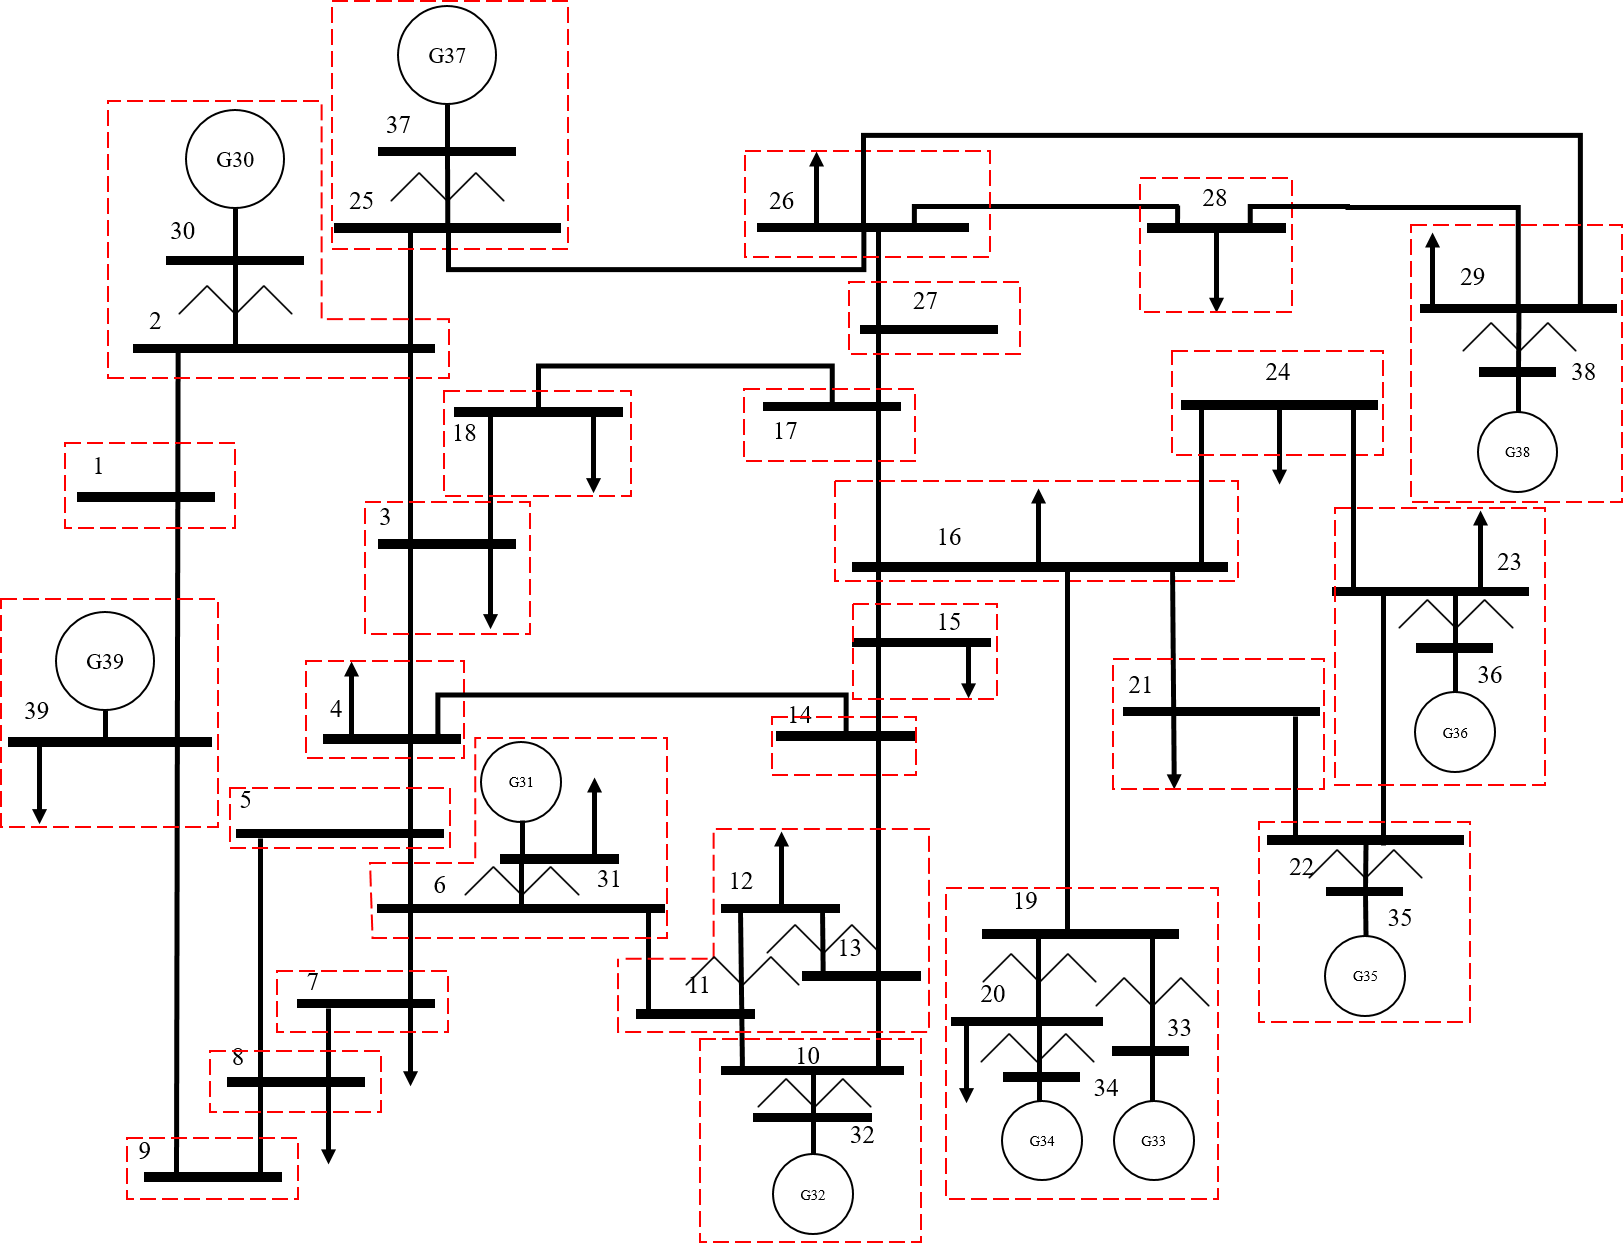
\includegraphics[width=\textwidth]{fig-ieee39.png}
	\caption{}\label{sfig:ieee-39}
	\end{subfigure}
	\begin{subfigure}{0.23\textwidth}
	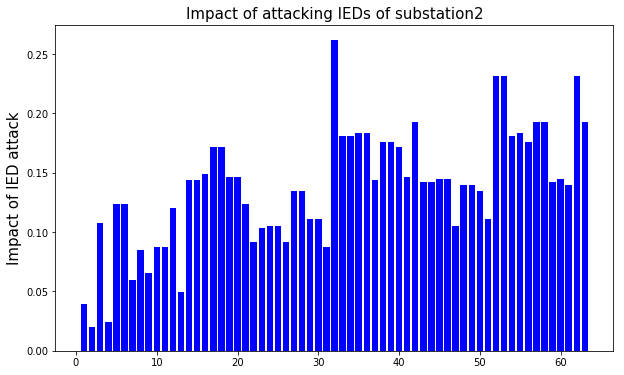
\includegraphics[width=\textwidth]{fig-sub2.png}
	\caption{}\label{sfig:sub-2}
	\end{subfigure}
	\caption{IEEE 39 bus system with 27 substation and impact of several attacks on IEDs of substation $2$.}
	\label{fig:physical}
\end{figure}

For modeling the physical system, the individual substations are required to be identified along with the associated IEDs. Thereafter, the possible combination of the IEDs are considered and contingencies are simulated based on these combinations. For example in Fig.~\ref{sfig:ieee-39} the substation with buses $2$ and $30$ has $6$ IEDs controlling the circuit breakers for generator G39, transformer HV and LV sides, and three transmission lines. There can be 63 combinations of these IEDs.

For each of these contingencies, a dynamic simulation is carried out for $10$ seconds. Therefore, the impact when an HMI is compromised and target IED set $\mathsf{S}$ is attacked can be evaluated as
\begin{equation}
I(\mathsf{S})=\beta_f\dfrac{\Delta f}{\Delta f_{\mathsf{rated}}}+\beta_v\frac{1}{N}\sum_{i=1}^{N}\dfrac{\Delta V_i}{\Delta V_{\mathsf{rated}}}
\end{equation} 
where $\Delta f$ and $\Delta V$ represent the maximum frequency and voltage deviation respectively and they are normalized to the rated deviations of $1\%$ and $5\%$ respectively. $\beta_f$ and $\beta_v$ are the suitable weighting factor and $N$ is the total number of buses in the system. Fig.~\ref{sfig:sub-2} shows the impact of $63$ possible contingencies when IEDs of substation $2$ are targeted. The impact has been calculated with $\beta_f=\beta_v=0.1$.

Let $\{\mathsf{S_1},\mathsf{S_2},\cdots,\mathsf{S_M}\}$ be the list of possible contingencies which can be created when the target vulnerability is compromised. The resulting risk ($R$) associated with the cyber attack on the target vulnerability $c$ is given by
\begin{equation}
R(c)=\zeta(c)\cdot\dfrac{1}{M}\sum_{i=1}^{M}\mathsf{S_i}
\end{equation}
The mean impact of all possible contingencies from a compromised HMI is considered as the measure of physical impact of the cyber attack. From Fig.~\ref{sfig:sub-2} the physical impact of compromising the HMI at substation $2$ is $0.138$. This is the mean impact of all the $63$ possible contingencies.